%%%%%%%%%%%%%%%%%%%%%%%%%%%%%%%%%%%%%%%%%
% Jacobs Landscape Poster
% LaTeX Template
% Version 1.1 (14/06/14)
%
% Created by:
% Computational Physics and Biophysics Group, Jacobs University
% https://teamwork.jacobs-university.de:8443/confluence/display/CoPandBiG/LaTeX+Poster
% 
% Further modified by:
% Nathaniel Johnston (nathaniel@njohnston.ca)
%
% This template has been downloaded from:
% http://www.LaTeXTemplates.com
%
% License:
% CC BY-NC-SA 3.0 (http://creativecommons.org/licenses/by-nc-sa/3.0/)
%
%%%%%%%%%%%%%%%%%%%%%%%%%%%%%%%%%%%%%%%%%

%----------------------------------------------------------------------------------------
%   PACKAGES AND OTHER DOCUMENT CONFIGURATIONS
%----------------------------------------------------------------------------------------

\documentclass[final]{beamer}

\usepackage[scale=1.0]{beamerposter} % Use the beamerposter package for laying out the poster
\usetheme{confposter} % Use the confposter theme supplied with this template

\setbeamercolor{block title}{fg=dblue!80,bg=white} % Colors of the block titles
\setbeamercolor{block body}{fg=black,bg=white} % Colors of the body of blocks
\setbeamercolor{block alerted title}{fg=white,bg=dblue!70} % Colors of the highlighted block titles
\setbeamercolor{block alerted body}{fg=black,bg=dblue!10} % Colors of the body of highlighted blocks
% Many more colors are available for use in beamerthemeconfposter.sty

%-----------------------------------------------------------
% Define the column widths and overall poster size
% To set effective sepwid, onecolwid and twocolwid values, first choose how many columns you want and how much separation you want between columns
% In this template, the separation width chosen is 0.024 of the paper width and a 4-column layout
% onecolwid should therefore be (1-(# of columns+1)*sepwid)/# of columns e.g. (1-(4+1)*0.024)/4 = 0.22
% onecolwid should therefore be (1-(# of columns+1)*sepwid)/# of columns e.g. 
% (1-(3+1)*0.025)/3 = 0.3
% Set twocolwid to be (2*onecolwid)+sepwid = 0.464
% Set threecolwid to be (3*onecolwid)+2*sepwid = 0.708

\newlength{\sepwid}
\newlength{\onecolwid}
\newlength{\twocolwid}
\newlength{\threecolwid}
\setlength{\paperwidth}{36in} % A0 width: 46.8in
\setlength{\paperheight}{48in} % A0 height: 33.1in
\setlength{\textwidth}{34in} % A0 width: 46.8in
\setlength{\textheight}{46in} % A0 height: 33.1in
\setlength{\sepwid}{0.025\paperwidth} % Separation width (white space) between columns
\setlength{\onecolwid}{0.3\paperwidth} % Width of one column
\setlength{\twocolwid}{0.625\paperwidth} % Width of two columns
\setlength{\threecolwid}{0.95\paperwidth} % Width of three columns
\setlength{\topmargin}{-0.5in} % Reduce the top margin size
%-----------------------------------------------------------

\usepackage{graphicx}  % Required for including images
\newcommand{\Cyclus}{\textsc{Cyclus}\xspace}%

\usepackage{tabularx}
\newcolumntype{b}{X}
\newcolumntype{s}{>{\hsize=.5\hsize}X}
\newcolumntype{m}{>{\hsize=.75\hsize}X}
\newcolumntype{z}{>{\hsize=.65\hsize}X}

\usepackage{booktabs} % Top and bottom rules for tables
\usepackage{xspace}

\usepackage{multirow}

\usepackage[acronym, toc]{glossaries}
\newacronym{NNL}{NNL}{National Nuclear Laboratory}
\newacronym{MA}{MA}{minor actinide}
\newacronym{DU}{DU}{depleted uranium}
\newacronym{LWR}{LWR}{Light Water Reactor}
\newacronym{MOX}{MOX}{Mixed Oxide Fuel}
\newacronym{FBR}{FBR}{Fast Breeder Reactor}
\newacronym{SFR}{SFR}{Sodium-cooled Fast Reactor}
\newacronym{FLM}{FLM}{Fuel Loading Model}
\newacronym{EFMC}{EFMC}{effective fissile mass coefficient}
\newacronym{ORNL}{ORNL}{Oak Ridge National Laboratory}
\newacronym{PWR}{PWR}{Pressurized Water Reactor}
\newacronym{FIT}{FIT}{Functionality Isolation Test}
\newacronym{MSR}{MSR}{Molten Salt Reactor}
\newacronym{PRISM}{PRISM}{Power Reactor Innovative Small Module}
\newacronym{UNF}{UNF}{Used Nuclear Fuel}
\newacronym{EPF}{EPF}{Equivalent Pu-239 Factor}
\newacronym{UNF-STANDARDS}{UNF-ST\&DARDS}{\gls{UNF} Storage, Transportation \& Disposal Analysis Resource and Data System}
\newacronym{PyNE}{PyNE}{Python for Nuclear Engineering}
\usepackage{tikz}
\usetikzlibrary{positioning, arrows, decorations, shapes }
% Define block styles
\tikzstyle{decision} = [diamond, draw, fill=blue!20, 
text width=4.5em, text badly centered, node distance=3cm, inner sep=0pt]


\tikzstyle{block} = [rectangle, draw, text centered, fill=blue!20]
\tikzstyle{line} = [draw, -latex']
\tikzstyle{cloud} = [draw, ellipse,fill=red!20, node distance=6em,
minimum height=2em]
\tikzstyle{process} = [rectangle, rounded corners, minimum width=2.5cm, minimum height=1cm,text centered, draw=black, fill=blue!30]
\tikzstyle{object} = [ellipse, rounded corners, minimum width=3cm, minimum height=1cm,text centered, draw=black, fill=green!30]
\tikzstyle{empty} =  [rectangle, rounded corners, minimum width=2.5cm, minimum height=0.7cm,text centered, draw=black, fill=white!30]
\tikzstyle{arrow} = [thick,->,>=stealth]


\usetikzlibrary{shapes.multipart}
\usetikzlibrary{positioning}


\setbeamertemplate{bibliography item}[text]

%----------------------------------------------------------------------------------------
%   TITLE SECTION 
%----------------------------------------------------------------------------------------

\title{Impact of Composition Approximation on Simulated Nuclear Fuel Cycle Metrics} % Poster title

\author{Jin Whan Bae$^{1}$, Joshua L. Peterson-Droogh$^{2}$, Kathryn D. Huff$^{1}$}
\institute{
$^{1}$ Dept. of Nuclear, Plasma, and Radiological Engineering, University of Illinois at Urbana-Champaign, Urbana, IL
\and
$^{2}$ Idaho National Laboratory, Idaho Falls, ID}
\date{}
%----------------------------------------------------------------------------------------

\begin{document}

\addtobeamertemplate{block end}{}{\vspace*{2ex}} % White space under blocks
\addtobeamertemplate{block alerted end}{}{\vspace*{2ex}} % White space under highlighted (alert) blocks

\setlength{\belowcaptionskip}{2ex} % White space under figures
\setlength\belowdisplayshortskip{2ex} % White space under equations

\begin{frame}[t] % The whole poster is enclosed in one beamer frame

\begin{columns}[t,totalwidth=\threecolwid] % The whole poster consists of three major columns, the second of which is split into two columns twice - the [t] option aligns each column's content to the top

\begin{column}{\sepwid}\end{column} % Empty spacer column

\begin{column}{\onecolwid} % The first column

%----------------------------------------------------------------------------------------
%   OBJECTIVES
%----------------------------------------------------------------------------------------

\begin{alertblock}{Objectives}

Compare the validity and limits of simplifying \gls{UNF} composition.
by comparing two \gls{UNF} inventories:
\begin{itemize}
    \item Detailed burnup and enrichment composition from database
    \item Averaged burnup and enrichment composition
\end{itemize}
\bigskip \bigskip

We compare:

\begin{itemize}
    \item Isotopic mass
    \item Waste management metric
    \item Equivalent $^{239}Pu$ Factor \cite{anon_plutonium_1989}
\end{itemize}

\end{alertblock}

%----------------------------------------------------------------------------------------
%   INTRODUCTION
%----------------------------------------------------------------------------------------

\begin{block}{Introduction}

\gls{UNF-STANDARDS} has been developed to integrate
a centralized \gls{UNF} database \cite{peterson_used_2013} and the SCALE suite of codes \cite{noauthor_scale_nodate} to
perform neutronics analysis for
\gls{UNF} management and disposal analysis.
This comprehensive, high-resolution database lists every \gls{UNF} assembly discharged 
in the U.S ($\sim244,896$) and their properties
(initial enrichment, burnup, ORIGEN-depleted isotopic composition, assembly type, etc.).
While high resolution of this kind is exceptionally valuable, the volume of data can 
present challenges for processing and simulation computation times.

We compare the predicted U.S. \gls{UNF} inventory in 2020 calculated using
\gls{UNF-STANDARDS} to the same prediction calculated using a simplified \gls{UNF} 
inventory assuming an average burnup and enrichment in order to assess the impact of this common simplifying assumption on fuel cycle metric accuracy.

\end{block}

%----------------------------------------------------------------------------------------
%   MATERIALS
%----------------------------------------------------------------------------------------

\begin{block}{Methods}

We compare the predicted U.S. \gls{UNF} inventory in 2020 calculated using
\gls{UNF-STANDARDS} to the same prediction calculated using a simplified \gls{UNF} 
inventory assuming an average burnup and enrichment in order to assess the impact of this common simplifying assumption on fuel cycle metric accuracy.

\begin{figure}
    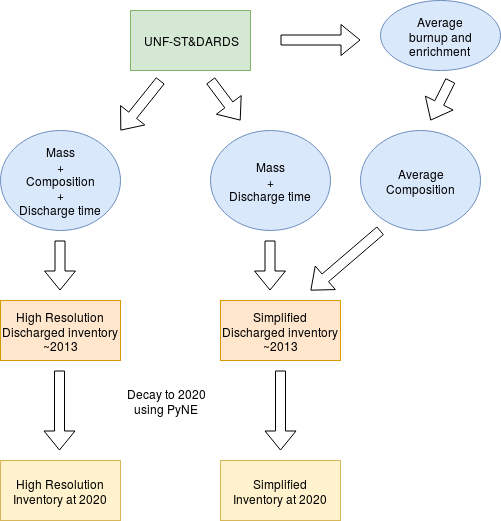
\includegraphics[width=0.85\textwidth]{../images/flow.png}
    \caption{Workflow for generating two \gls{UNF} inventories using \gls{UNF-STANDARDS}}
    \label{fig:flow}
\end{figure}

\end{block}

\begin{block}{Metrics}

\gls{UNF} is typically either destined for disposal (after storage) or reprocessing.
Accordingly, the U.S. \gls{UNF} inventory can be analyzed in two different
ways, with certain metrics important for each.

\begin{table}[h]
    \centering
    \begin{tabular}{ccc}
        \hline
        Analysis type & Important metric & Unit\\
        \hline
        Fuel cycle analysis & Equivalent Pu-239 \cite{anon_plutonium_1989} & t \\
        \hline
        \multirow{2}{*}{Waste management} & \shortstack{Decay heat \\ (@ 2020, 2100, 3100)} & MW\\
        & \shortstack{Activity \\ (@ 2020, 2100, 3100)} & Bq \\
        \hline
    \end{tabular}
    \caption{Important metrics for \gls{UNF} with regard to analysis types }
    \label{tab:met}
\end{table}

The relative difference values are calculated using the following formula:
\[\text{Rel. Error} = \frac{M_{HR} - M_{s}}{M_{HR}}\]
\[M_{HR} = \text{Metric in inventory (high-resolution case)}\]
\[M_{S} = \text{Metric in inventory (simplified case)}\]

\end{block}

%----------------------------------------------------------------------------------------

\end{column} % End of the first column

\begin{column}{\sepwid}\end{column} % Empty spacer column


%----------------------------------------------------------------------------------------

\begin{column}{\onecolwid} % The second column

%----------------------------------------------------------------------------------------
%   IMPORTANT RESULT
%----------------------------------------------------------------------------------------


%----------------------------------------------------------------------------------------
%   RESULTS
%----------------------------------------------------------------------------------------



\begin{block}{Average Composition}
The average assembly has:
\begin{itemize}
    \item 36.169 GWD/MTHM burnup
    \item 3.39\% $^{235}U$ Enrichment
\end{itemize}

\begin{table}[h]
    \centering
    \begin{tabular}{cr}
        \hline
        Isotope & wt \% \\
        \hline
        $^{238}U$ & 96.5000 \\
        $^{235}U$ & 1.0400 \\
        $^{241}Am$ & 0.0160 \\
        $^{239}Pu$ & 0.7550   \\
        $^{137}Cs$ & 0.1320   \\
        ${90}Sr$ & 0.0552  \\
        Pu Total & 1.2760   \\
        \hline
    \end{tabular}
    \caption{Composition of the representative
             assembly selected for analysis.}
    \label{tab:avg}
\end{table}

\end{block}

\begin{block}{PyNE and ORIGEN Decay Calculation Comparison}
To ensure the validity of the decay function implemented in \gls{PyNE}, 
we imported the database into \gls{PyNE} and decayed each assembly
to 2020.

\begin{table}[h]
    \centering
    \begin{tabular}{l|rr|r}
        \hline
        Metric & PyNE & ORIGEN & $\Delta \%$ \\
        \hline
        $^{239}Pu$ mass [t] & 520.52 & 520.50 & 3.8E-05\\
        $^{137}Cs$ mass [t] & 59.23 & 59.19 & 6.7E-04\\
        $^{235}U$ mass [t] & 771.42 & 771.39 & 3.8E-05\\
        Total mass [t] & 68,072 & 67,984 & 1.2E-03\\
        Decay Heat [MW] & 61.31 & 61.10 & 3.4E-03 \\
        Activity [Bq] & $6.76e20$ & $6.74e20$ & 2.9E-03 \\
        \hline
    \end{tabular}
    \caption{Comparison between \gls{PyNE} decayed and ORIGEN decayed \gls{UNF} inventory in 2020.}
\end{table}
\end{block}


\begin{block}{Isotopic Mass}

\begin{figure}
    \centering
    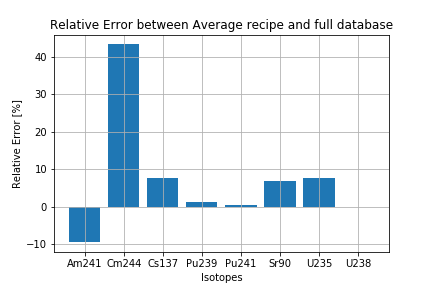
\includegraphics[width=0.7\textwidth]{../images/iso_rel.png}
    \caption{Relative error between high resolution and simplified case for different isotopes.}
    \label{fig:iso_rel}
\end{figure}


\begin{figure}
    \centering
    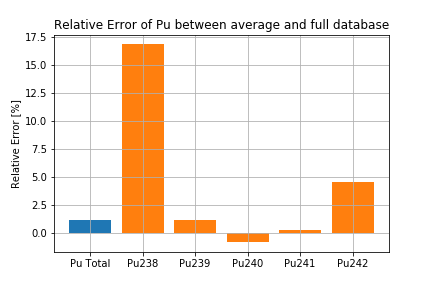
\includegraphics[width=0.7\textwidth]{../images/pu_rel.png}
    \caption{Relative error between high resolution and simplified case for plutonium isotopes.}
    \label{fig:pu_rel}
\end{figure}
\end{block}


\begin{block}{Waste Management Metrics}
The two major waste management metrics are radioactivity and
decay heat. Since the two metrics change in time, the metrics
are evaluated in time.

\begin{figure}
    \centering
    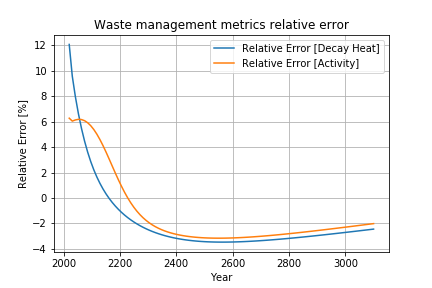
\includegraphics[width=0.8\textwidth]{../images/ha_err.png}
    \caption{Relative error of activity and decay heat of the
            \gls{UNF} inventory over time.}
    \label{fig:wm_err}
\end{figure}


\end{block}

\end{column} % End of the first column

\begin{column}{\sepwid}\end{column} % Empty spacer column


%----------------------------------------------------------------------------------------

\begin{column}{\onecolwid} % The second column


\begin{block}{Fuel Cycle Analysis Metrics}
Given the isotopic compositions of the \gls{UNF} profile in 2020,
we calculate the equivalent $^{239}Pu$ for both cases, for
both spectra.

\begin{table}[h]
    \centering
    \begin{tabular}{ccc}
        \hline
        Category & Equiv. $^{239}Pu$ ton & Rel. Error [\%] \\
        \hline
        HR thermal & 880.5 & \multirow{2}{*}{7.28}\\
        Simplified thermal & 816.4\\
        \hline
        HR fast & 1214.0 & \multirow{2}{*}{4.67}\\
        Simplified fast & 1157.3 &\\
        \hline
    \end{tabular}
    \caption{Equivalent $^{239}Pu$ ton value comparison for High-resolution and simplified case.}
    \label{tab:equiv}
\end{table}


To explain this error, we plotted every assembly and its
normalized equivalent $^{239}Pu$, shown in Figures \ref{fig:fast_all} and \ref{fig:thermal_all}.

\[ \widetilde{^{239}Pu_{equiv}} = \frac{^{239}Pu_{equiv}}{M_{assem}}\]

\begin{figure}
    \centering
    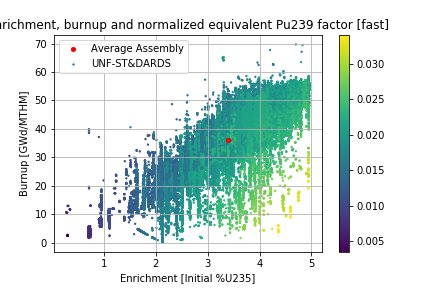
\includegraphics[width=0.8\textwidth]{../images/fast_all.png}
    \caption{All assemblies in the database and their normalized equivalent Pu-239 in a fast reactor.}
    \label{fig:fast_all}
\end{figure}

\begin{figure}
    \centering
    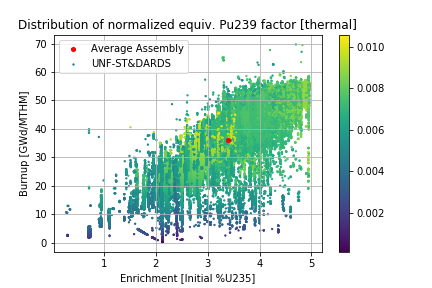
\includegraphics[width=0.8\textwidth]{../images/thermal_all.png}
    \caption{All assemblies in the database and their normalized equivalent Pu-239 in a thermal reactor.}
    \label{fig:thermal_all}
\end{figure}
\end{block}
%----------------------------------------------------------------------------------------
%   CONCLUSION
%----------------------------------------------------------------------------------------

\begin{alertblock}{Conclusion}
We compared the simplified \gls{UNF}
inventory and the high-resolution \gls{UNF} inventory
at 2020 by calculating the isotopic differences as well
as important metrics for waste management and fuel cycle analysis. Results show:
\bigskip \bigskip

Simplified inventory is \textbf{not adequate} for waste management analysis
    \begin{itemize}
        \item Large error in FP and MA inventory
        \begin{itemize}
            \item FP and MA sensitive to initial enrichment and burnup
            \item FP and MA contributor in decay heat and activity
        \end{itemize}
        \item Discrete modeling for assemblies in repository modeling
    \end{itemize}
\bigskip \bigskip

Simplified inventory is \textbf{acceptable approximation} for fuel cycle analysis
    \begin{itemize}
        \item \textasciitilde 5\% error for $^{239}Pu_{equiv}$
        \item Reduces computational burden for fuel cycle simulators
    \end{itemize}
\end{alertblock}

%----------------------------------------------------------------------------------------
%   ACKNOWLEDGEMENTS
%----------------------------------------------------------------------------------------

\setbeamercolor{block title}{fg=norange,bg=white} % Change the block title color

\begin{block}{Acknowledgements}
The work done was funded through the Nuclear Engineering Science
Laboratory Synthesis (NESLS) program. We thank Kaushik Banerjee
from Oak Ridge National Laboratory for providing the data used
in this paper. 

\end{block}

%----------------------------------------------------------------------------------------
%   CONTACT INFORMATION
%----------------------------------------------------------------------------------------

\setbeamercolor{block alerted title}{fg=black,bg=norange} % Change the alert block title colors
\setbeamercolor{block alerted body}{fg=black,bg=white} % Change the alert block body colors



\begin{alertblock}{Contact Information}
\setbeamercolor{block title}{fg=norange,bg=white} % Change the block title color
\begin{itemize}
    
    \item Web: \href{arfc.github.io}{arfc.github.io}
    \item Email: \href{mailto:jbae11@illinois.edu}{jbae11@illinois.edu}
    \item Phone: +1 (217) 377-5784
\end{itemize}

\end{alertblock}

%----------------------------------------------------------------------------------------

\end{column} % End of column 2

\begin{column}{\sepwid}\end{column} % Empty spacer column

\begin{column}{\onecolwid} % The third column


\begin{block}{References}

        {\footnotesize\bibliographystyle{abbrv} 
        \bibliography{poster}}
\end{block}


%----------------------------------------------------------------------------------------



\end{column} % End of the third column

\end{columns} % End of all the columns in the poster

\end{frame} % End of the enclosing frame

\end{document}
\begin{column}{\sepwid}\end{column} % Empty spacer column
